\documentclass{article}
\usepackage{amsmath}
\usepackage{amssymb}
\usepackage{graphicx}
\usepackage{anysize} %<-for setting margins
\marginsize {1.6cm}{1.6cm}{2.0cm}{2cm}
\usepackage{color}
\newcommand{\dean}[1]{\textsf{\emph{\textbf{\textcolor{red}{#1}}}}}

\title{Response To Reviews - A Data-Driven Framework for Neural Field Modeling}
\author{D. Freestone, P. Aram, M. Dewar, K. Scerri, D. Grayden, V. Kadirkamanathan}

\begin{document}
    \maketitle
    
    \section{Reviewer 1}
    
        We first address the reviewer's main concerns, followed by the reviewer's additional comments.
        
    \subsection{Main Concerns}
    It would be useful to mention the above (now below) explicitly in the introduction and try to address them in later sections of the paper.

    \begin{enumerate}
        \item Do not use real data for the validation of their approach

	\emph{The authors appreciate that the only way to truly validate the proposed framework is with real data. However, before validating the method on real data we believe that it is important to first validate the method artificial data, where the true and estimated parameters can be compared. Given the space limitations on the article, it is not feasible to show examples using real data in this paper. Another paper demonstrating the application of the method with data recorded from a Utah array implanted in an epilepsy surgical patient is currently in preparation. In an effort to make the method employed in the paper more explicit, we have added ``To illustrate the estimation framework, data is generated using the neural field equations incorporating modeled sensors enabling a comparison between the estimated and true parameters'' to the introduction.}
	
        \item Assume that a few kernel basis functions accurately represent the actual connectivity kernel, which might not be the case when using real data;

	\emph{The examples presented in the paper use the Mexican hat connectivity kernel. The framework is also valid for other connectivity kernels provided they are homogeneous and that they can be approximated by a set of isotropic basis functions parametrized by a coefficient vector $\mathbf{\theta}$. The mathematical formulation does not restrict the shape of the kernel, where anisotropic (we assume isotropy of the kernel basis functions to make the simplification in equation~18) arbitrary shapes can be represented. Furthermore, the kernel basis functions need not be a Gaussian shape, but can be, for example, Laplacian to describe the ``wizard hat'' connectivity or B-spline functions to describe a kernel with a more compact support. For more complex basis functions some of the analytic derivations described in the Appendix may have to be performed numerically. We have added the above statements to the methods section (after equation~13) to be more explicit in describing subtleties of the method.}

        \item Do not consider the EEG/MEG lead field when constructing their mapping between the membrane voltage and the electrophysiological data (observation function)

	\emph{In response to this important point, the authors have made an effort to be clear that we are not considering scalp EEG to be a valid data source for the estimation framework. Amendments have been made to the Introduction (last paragraph), Method (after equation 9), and Discussion. We have primarily developed the framework for higher density intracranial measurements. We believe that the spatial frequency response and sampling density of extracranial EEG/MEG measurements will be insufficient to estimate the connectivity structure.}
	
	
    \end{enumerate}
    
    \subsection{Additional Comments}
    
    \begin{enumerate}
        \item The discrepancy of the results in Experiment II where the weights of the basis functions are not in agreement with the actual parameters while the reconstructed kernels seem satisfying.

        \item The use of Euler discretisation and how this affects the system's behavior.

		\emph{This point was made by a reviewer from our PLoS attempt. The reviewer stated: ``1. The authors might want to reference prior work in using Kalman
		Filtering for the estimation of neural mass models from data [1-3],
		[13]. In fact from those papers stressed the importance of carrying out
		a high order discretization of the differential equations, which should
		be in fact treated as stochastic. In equation (S1.1) of the extended
		derivation, it is shown that an Euler approximation is taken which may
		even change the dynamical properties of the system. The authors should
		discuss this issue.'' ALL THESE PAPERS USE a method called local linearisation approach for discretisation.}
		
        \item The derivation of Equations (30) and (31) [spacing of basis functions] and make them more transparent for the general audience.

\emph{This appendix provides a derivation for equations ?? and ??. The derivation is adapted from (Sanner et al., 1992, and Scerri et al., 2009). Consider the cortical sheet defined on the surface $\Omega$ with the sensors placed on a regular grid at positions $\mathbf{r}_n$ (where $n=0,...,n_y-1$ indexes the sensors) that are separated by the distance $\Delta_y$. The observations can be considered samples from a continuous field that is filtered (convolved) with the observation kernel described by
\begin{equation}
	y(\mathbf{r}_n)=\sum_{n=0}^{n_y-1}\delta(\mathbf r - \mathbf{r}_n ) v_m(\mathbf{r}),
\end{equation} 
where $v_m(\mathbf{r}) = v_t(\mathbf{r})\ast m(\mathbf{r})$. The Fourier transform of $y(\mathbf{r}_n)$ is
\begin{align}
 Y(\boldsymbol{\nu}) &= \frac{1}{\Delta_y^2}\sum_{n=0}^{n_y-1} \delta\left(\boldsymbol{\nu}-\frac{n}{\Delta_y}\right) \ast V_m(\boldsymbol \nu) \\
	&= \frac{1}{\Delta_y^2}V_m(\boldsymbol\nu)+\frac{1}{\Delta_y^2}\sum_{n=1}^{n_y-1} V_m\left(\boldsymbol{\nu}-\frac{n}{\Delta_y}\right).
\end{align} 
It should be clear that $Y(\boldsymbol{\nu})$ contains $V_m(\boldsymbol\nu)$ plus $n_y-2$ copies (aliases) of $V_m(\boldsymbol\nu)$ repeated on the regular lattice centered at $n\Delta_y^{-1}$. Due to the lowpass action of the observation kernel, the filtered dynamic field is band-limited with a cutoff frequency $\boldsymbol\nu_{cy}$. In order for $V_m(\boldsymbol\nu)$ to be disjointed from its aliases, the amount of shift $\Delta_y^{-1}$ must be at least $2\boldsymbol\nu_{cy}$, since each alias has a spectral range of
\begin{equation}
	\boldsymbol\nu = \left[\frac{n}{\Delta_y}-\boldsymbol{\nu}_{cy},\frac{n}{\Delta_y}+\boldsymbol{\nu}_{cy}\right].
\end{equation}
Therefore, to avoid aliasing the distance between observations must satisfy
\begin{equation}\label{eq:SamplingCriteria}
	\frac{1}{\Delta_y} \ge 2\nu_{cy}.
\end{equation}
Since the observation kernel is not an ideal filter an oversampling parameter should be included to further separate the aliases. Rearranging equation~\ref{eq:SamplingCriteria} and adding the oversampling parameter, $\rho$, gives
\begin{equation}\label{ap:Shannon}
	\Delta_y\le\frac{1}{2\rho\nu_{cy}},
\end{equation}
where $\rho \in \mathbb{R} \ge 1$. }

        \item The existing literature on inversion schemes for similar models of brain activity.
        \item In section 3, Table 6 is mentioned however there is no such table in the ms.
    \end{enumerate}
    
    \section{Reviewer 2}
    
    We thank the author for their encouraging review. Each point raised is dealt with in turn.

\begin{enumerate}
    \item The handling of the (to borrow a term from numerical weather forecasting) `sub-grid scale physics' is inadequate for nervous systems (see, e.g., equation 8 [The nonlinear IntegroDifference Equation]). I do very much appreciate the spectral estimation of spatial and temporal scales. But the model errors are lumped into an iid model error term that is not realistic. For instance, the flow of potassium in the extracellular spaces has a known dynamic that will affect network excitability, generating important sub-grid dynamics that is anything but iid. See, for instance, the example in Ullah et al PLoS Comp Biol 2010 where without such dynamics, state tracking and parameter estimation for a neural system fails. A beautiful overview of sub-grid effects in data assimilation is found in Kalnay's 2003 book. I would very much value the authors comments on these issues. I guess were I to respond to this question, that I might consider extending the model error term to an autoregressive model. But I will let the authors answer this question.\\

    \emph{talk about model order}

	\emph{Indeed, there will always be a mismatch between a mathematical model and the natural phenomena it is attempting to describe. The model proposed in our paper is modest in terms of the temporal dynamics, where the state transition is assumed to be first-order. However, the development of the framework for this modest brain model is a significant development that can be expanded to include longer range time dependencies. A major benefit in using a mean field model is the freedom to lump detailed parameters, such as specific ion concentrations, into more general parameters such as the connectivity kernel coefficients that describe the net system gain. Please note, we have assumed that factors influencing excitability are stationary over the estimation period. This is a reasonable assumption is applying the framework to an evoked potential experiment. An extension to our framework, that is currently in development, is to allow for time-varying parameter estimates. This will allow the application of the framework to longer-term data recordings. The problem then can be posed in terms of convergence time and estimation accuracy vs. nonstationarity of the metabolic processes and other unmodeled brain dynamics.}
	
	
\item Although we all know the 1970s version of Wilson and Cowan's field equations, there was an intriguing stochasticization of these equations by Benayoun et al PloS Comp Biol 2010. I and others will value the authors' thoughts of how a more palatable stochasticization of these field equations might influence the future development of the data-assimilation framework presented in this paper.

\item This is NeuroImage, not the Physical Review. Although most of this framework involves mathematics that is reasonable to follow for typical readers of this journal, I would suggest that the authors explain and expand a bit on the introduction of Green's functions where introduced in equation 6.\\

\emph{The synaptic response kernel can be viewed as the Green function of a linear differential equation defined by the differential operator $\textrm{D}=d/dt + \zeta$ i.e., satisfying
\begin{equation}
	\label{GreensFuncDef} \textrm{D}h\left( t \right) = \delta \left( t \right), 
\end{equation} 
where $\delta(t)$ is the Dirac-delta function. Applying the differential operator $\textrm{D}$ on equation (5) from the main text we have
\begin{align}
 \textrm{D}v\left(\mathbf r,t\right)&= \textrm{D}\left(h\ast g\right)\left(\mathbf r,t\right)\\
&=\left(\textrm{D}h\ast g\right)\left(\mathbf r,t\right)\\
&=\left(\delta \left(t\right)\ast g\right)\left(\mathbf r,t\right)\\
&=g\left(\mathbf r,t\right)
\end{align}
where $\ast$ denotes convolution operator. This gives the standard form of the model
\begin{equation}
	\label{FinalFormContinuous} 
	\frac{dv\left( \mathbf{r},t \right)}{dt} + \zeta v\left( \mathbf{r},t \right) = \int_\Omega {w\left( \mathbf{r},\mathbf{r}' \right)f\left( {v\left( \mathbf{r}',t \right)} \right)\, d\mathbf{r}'}. 
\end{equation}}

\item What is the relation of the substitution of the temporal and spatial basis functions as employed in this paper to Galerkin's projection? How do the two techniques differ? If this is close, the non-local case for a Galerkin projection (typically used in diffusive processes) has not, to my knowledge, been done. Certainly not in a way that is obvious for neural field theory. Perhaps this is my ignorance. This seems important to clarify for the rest of us.
\item In the isotropic and translationally invariant case examined here, would a Fourier basis for temporal and spatial structure have been a formally correct alternative?\\

\emph{Gaussians has semi-compact support but Fourier basis functions are global functions. Gaussian can be easily extended to higher dimension (don't know about the Fourier basis functions), any orthonormal basis functions like Fourier basis functions simplify our equations, $\Gamma$ becomes identity matrix, but using Gaussian basis functions equations are in their generic form.}

\item In equation 29, what would a reasonable $v_c$ be for a real neuronal system (mammalian) given the number of neurons and scale of electrodes? I am concerned that it might be much higher than any of us wish to consider. One would perhaps be saved by the filter characteristics of brain (e.g. Phys. Rev. E 73, 051911 (2006)).
\item The two covariance inflation parameters in equation 41 make me cringe. How are we best to adjust these fudge factors?
\emph{The positive constant $\alpha$ determines the spread of the sigma points around $\mathbf{\bar x}$ which can be made arbitrary small (e.g. $0<\alpha\le 10^{-4} $) to minimise higher order effect (cite Julier (The Scaled Unscented Transformation) and  Haykin (Kalman filtering and neural network) , and  $\kappa$ is an additional scaling parameter which is usually set to $3-n_x$. cite Julier A New Approach for Filtering Nonlinear Systems}



\item I understand that the Mexican Hat bases are in this paper often a composite of $\theta_0$, $\theta_1$, and $\theta_2$, representing short range excitation, short range inhibition, and long range excitation. But many will be confused by this subtlety, and at times in the text the Mexican Hat basis is described as if it were a single function. I would show how the theta's sum to create the general spatial basis shape of the hat in figure 1, and go through the paper in order to clarify this issue.\\
\emph{I think we need to show each kernel basis function in Figure 1}
 \begin{figure*}[!ht]
 \begin{center}
 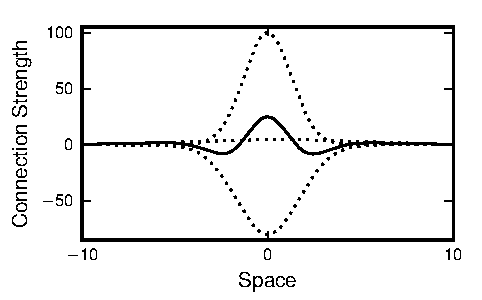
\includegraphics{./Graph/pdf/fig1_revised.pdf} 
 \end{center}
 \caption{}
 \label{fig:Figure1}
 \end{figure*}

\item A few comments on how to adapt the smoother for real time implementation would be helpful. I presume that one would perform the smoothing during a training phase. But one would also wish to adapt in real time as observation or control scenarios progressed. A few words of perspective would be invaluable to help others translate the author's wisdom on this method to other applications.
\item Figure 4. Should the axes be indicated as spatial frequency rather than just Hz?
\item Page 45, Appendix D, Par 1, line 6: should `transform of a n-' should be `transform of an n-' ? I am grammatically challenged perhaps.
\end{enumerate}

\end{document}